\documentclass[11pt]{article}
\usepackage{icmlko}
\begin{document}

\title{용량은 자루로 못 쪼갠다 --- 실패한 처방이 축 하나를 확정했다}
\author{월드모델 실험실}
\date{노트 409 · 2026년 8월 1일}
\maketitle

\begin{abstract}
노트 408이 문제를 하나 남겼다 --- 도메인마다 원하는 용량이 다르고
\textbf{웹툰만 반대 방향}인데 판 무게가 21\% 다. 전역 깊이 하나는 늘
타협이다. 처방: F18 은 이미 자루를 서른둘 친다. \textbf{자루마다 깊이를
$4 \cdot 6 \cdot 8$ 로 돌리면} 도메인별 매개변수를 하나도 안 늘리고
도메인마다 다른 용량을 줄 수 있지 않을까. 원핫과 달리 \textbf{안 본
도메인에도 그대로 간다}.

\textbf{미리 적은 실패 조건 그대로 걸렸다}: \emph{배깅은 예측을 평균할 뿐
도메인이 자기에게 맞는 자루를 고르지 못한다.} 짝 12뽑기 판
$\mathbf{-0.0007 \cdot 2/12}$ --- 조건 ① 로 유지. \textbf{안 바꿨다.}

그런데 도메인별로 보면 \textbf{정확히 거울}이다.

\begin{center}
\begin{tabular}{lrrr}
\hline
 & 깊이 $4{\to}6$ & lr $.06{\to}.10$ & \textbf{자루 섞기} \\
\hline
아이돌 & $+0.1179$ & $+0.0440$ & $\mathbf{-0.0306}$ \\
펀딩 & $+0.0409$ & $+0.0091$ & $\mathbf{-0.0124}$ \\
$\cdots$ & & & \\
팝업 & $-0.0050$ & $-0.0009$ & $\mathbf{+0.0100}$ \\
웹툰 & $-0.0241$ & $-0.0150$ & $\mathbf{+0.0086}$ \\
\hline
\end{tabular}
\end{center}

$\rho = \mathbf{-0.808}$ (깊이와) · $\mathbf{-0.854}$ (lr 과). 용량을
원하던 도메인이 섞으면 잃고, 싫어하던 도메인이 번다. \textbf{섞기는 평균
용량을 줄 뿐이다.}
\end{abstract}

\section{실패가 확정한 것}

노트 408은 두 손잡이(깊이 · lr)가 $\rho{=}{+}0.679$ 로 같은 순서를 만든다고
적으면서 ``설명은 없고 규칙만 있다''고 했다. 손잡이 둘은 둘 다
\textbf{같은 종류}(전역 용량)라 상관이 높은 것이 당연할 수 있었다.

자루 섞기는 \textbf{다른 기계}다 --- 용량을 올리지도 내리지도 않고
\emph{섞는다}. 그 다른 기계가 같은 순서를 $|\rho| \approx 0.83$ 으로
다시 만든다. \textbf{기계 셋이 같은 순서를 만들면 그것은 손잡이의 성질이
아니라 도메인의 성질이다.}

용량 선호 순서(깊이 $4{\to}6$ 기준):
\begin{center}
아이돌 $\gg$ 펀딩 $>$ 모바일 $\approx$ 게임 $\approx$ 애니 $>$
도서 $\approx$ 시장팝업 $\approx$ 세계애니 $>$ 만화 $>$ 팝업 $>$ 웹툰
\end{center}

그리고 여전히 \textbf{크기가 아니고}(노트 408: 유보와 $\rho \approx 0$)
\textbf{원핫 아쉬움도 아니다}(노트 408: $\rho = +0.300$). \textbf{설명
후보가 셋째로 죽은 채 축만 단단해졌다.}

\section{왜 섞기가 안 되나}

배깅은 $\frac{1}{K}\sum_k f_k$ 를 낸다. 도메인 $d$ 에 깊은 나무가 맞고
도메인 $e$ 에 얕은 나무가 맞아도, \textbf{두 도메인이 같은 평균을 받는다}.
도메인이 자기에게 맞는 자루에 무게를 더 줄 방법이 없다. 그래서 결과가
깊이 $4 \cdot 6 \cdot 8$ 의 \emph{중간}이 되고, 중간에서 멀리 있던
도메인일수록 크게 움직인다 --- 그게 거울의 정체다.

도메인별 용량을 정말 주려면 \textbf{자루에 도메인 의존 무게}가 있어야
하는데, 그 무게는 안 본 도메인에서 정의되지 않는다. \textbf{원핫이 걸렸던
바로 그 벽}(노트 398--401)이 여기서도 같은 자리에 있다.

\section{남은 것}

\begin{tabular}{lp{7.2cm}}
\hline
용량 축의 정체 & 기계 셋이 확정했는데 설명이 셋 다 죽었다(크기 · 원핫
아쉬움 · 표시자 순도). 도메인의 무엇인가 \\
웹툰 & 축의 한쪽 끝에 혼자 있고 판 무게 21\% 다. 웹툰이 왜 얕은 것을
원하는지가 축을 푸는 열쇠일 수 있다 \\
안 본 도메인에서 정의되는 용량 & 도메인 의존 무게는 못 쓴다. 축 분포에서
용량을 읽는 방법이 있어야 한다 \\
\hline
\end{tabular}

\begin{figure}[h]
\centering
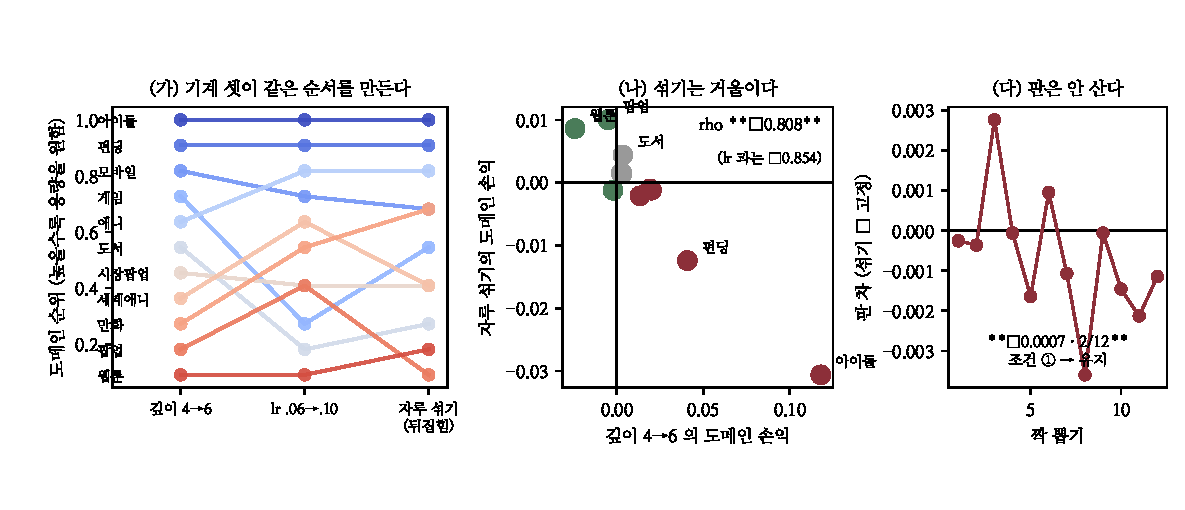
\includegraphics[width=\textwidth]{figs/fig409.pdf}
\caption{(가) 기계 셋(깊이 · lr · 섞기 뒤집음)이 만드는 도메인 순위.
(나) 섞기는 깊이의 거울 ($\rho = -0.808$). (다) 판은 안 산다 ---
$-0.0007 \cdot 2/12$.}
\end{figure}

\end{document}
